\documentclass[12pt]{article}
\usepackage[margin=0.915in]{geometry}

%%%
%%%             BEGIN Damian Preamble
%%%   Preface commands for pdfLaTeX output
%%%

%%
%% Calling relevant packages
%%

\usepackage[%
pdfstartview={FitV},
colorlinks=true,
menucolor=DarkGray,
linkcolor=MidnightBlue,
citecolor=MidnightBlue,
urlcolor=OrangeRed]{hyperref}
\usepackage{graphicx}
\DeclareGraphicsExtensions{.pdf}

%% From pandoc default: Begin
\usepackage{graphicx}
\makeatletter
\def\maxwidth{\ifdim\Gin@nat@width>\linewidth\linewidth\else\Gin@nat@width\fi}
\def\maxheight{\ifdim\Gin@nat@height>\textheight\textheight\else\Gin@nat@height\fi}
\makeatother
% Scale images if necessary, so that they will not overflow the page
% margins by default, and it is still possible to overwrite the defaults
% using explicit options in \includegraphics[width, height, ...]{}
\setkeys{Gin}{width=\maxwidth,height=\maxheight,keepaspectratio}
 %% From pandoc default: Begin

%\usepackage[hyper]{apacite}
\usepackage[svgnames]{xcolor}
\usepackage{rotating,bm,amsmath,amsfonts,amssymb,indentfirst,lscape,fancybox,fancyvrb,listings,pdfpages}
\usepackage[pagestyles]{titlesec}
%\usepackage{ucs}

%%
%% Format changes for chapter and section commands
%%

%\input{onesidedheader.tex}

%%
%% Chapter declarations
%%


%%
%% Section declarations
%%

%%
%% Subsection declarations
%%


%%
%% Subsubsection declarations
%%

%%
%% Listings setup information
%%

\lstset{language=R, frame=ltrb, framesep=5pt, xleftmargin=12pt, xrightmargin=5pt,
       numbers=none, breaklines=true, fancyvrb=true,
       breakatwhitespace=true, captionpos=b, abovecaptionskip=1.5ex,
       backgroundcolor=\color{Cornsilk},
       basicstyle=\small\color{DarkSlateGrey},
       keywordstyle=\ttfamily\color{DarkSlateGrey},
       identifierstyle=\ttfamily\color{DarkSlateGrey}\bfseries,
       commentstyle=\color{Fuchsia},
       stringstyle=\ttfamily,
       showstringspaces=false}

%%
%% Header and Footer Specification
%% TO ACTIVATE THE HEADER/FOOTER, ONE MUST PLACE \pagestyle{plain}
%% followed by \pagestyle{damian} in the document
%%

\widenhead{0.14in}{0.14in}

\renewpagestyle{plain}{}

\newpagestyle{damian}[\sffamily]{
\headrule
\sethead[\sectiontitle][\chaptertitle][\thepage]
  {\sectiontitle}{\chaptertitle}{\thepage}

\footrule
\setfoot[][\raisebox{-.85ex}[0pt]{\NavigationBar}][]
{}{\raisebox{-.85ex}[0pt]{\NavigationBar}}{}
	\newcommand{\NavigationBar}{%
	  \Acrobatmenu{PrevPage}{Previous}\hspace{.5cm}
	  \Acrobatmenu{NextPage}{Next}\hspace{.5cm}
	  \Acrobatmenu{FirstPage}{First}\hspace{.5cm}
	  \Acrobatmenu{LastPage}{Last}\hspace{.5cm}
	  \Acrobatmenu{GoBack}{Back}\hspace{.5cm}
	  \Acrobatmenu{Quit}{Quit}%
}
}

%%
%% Custom specifications, commands, and colors
%%

\definecolor{DarkGray}{cmyk}{0,0,0,.624}
\newcommand{\R}{{\sffamily \textup{R}}}
\newcommand{\MlwiN}{{\sffamily \textup{MlwiN}}}
\newcommand{\Sweave}{{\sffamily \textup{Sweave}}}
\newcommand{\sssty}{\scriptscriptstyle}
\newcommand{\bigdot}{\ensuremath{\hspace{-.3ex}\bm{.}\hspace{-.05ex}}}
\renewcommand{\abstractname}{Executive Summary}
\renewcommand{\lstlistingname}{\R~Code Example}
\renewcommand{\arraystretch}{1.2}
\setlength{\fboxsep}{4mm}
\setlength{\fboxrule}{0.4pt}

%%
%%		END Damian Preamble
%%

\hypersetup{%
  pdftitle={ Demonstration Skip Year SGP Analyses },
  pdfauthor={  Damian W. Betebenner  ,  Adam R. VanIwaarden  },
  pdfcreator={ Damian W. Betebenner  , Adam R. VanIwaarden  },
  pdfkeywords={},
  bookmarks=true} % pdfproducer={pdfLaTeX}

\usepackage{caption}
\usepackage{float}
\usepackage{longtable}
\usepackage{booktabs}
\usepackage{subcaption}
\usepackage{dcolumn}
\usepackage[bottom]{footmisc}

\setcounter{secnumdepth}{3}




%\usepackage{pdfdraftcopy}
\newtheorem{proposition}{Proposition}
\newtheorem{theorem}{Theorem}
\newtheorem{definition}{Definition}
\newtheorem{corollary}{Corollary}
\DeclareMathOperator*{\argmin}{arg\,min}

% \usepackage{bbm}
\DeclareMathAlphabet{\mathbbm}{U}{bbm}{m}{n}
\SetMathAlphabet\mathbbm{bold}{U}{bbm}{bx}{n}
\DeclareMathAlphabet{\mathbbmss}{U}{bbmss}{m}{n}
\SetMathAlphabet\mathbbmss{bold}{U}{bbmss}{bx}{n}
\DeclareMathAlphabet{\mathbbmtt}{U}{bbmtt}{m}{n}

\providecommand{\tightlist}{% Error in pandoc - http://tex.stackexchange.com/questions/257418/error-tightlist-converting-md-file-into-pdf-using-pandoc
  \setlength{\itemsep}{0pt}\setlength{\parskip}{0pt}}


\newcommand{\pl}[1]{\textsf{PL#1}}
\newcommand{\Cov}{\ensuremath{\mbox{\textsf{Cov}}}}
\newcommand{\Diag}{\ensuremath{\mbox{\textsf{Diag}}}}
\newcommand{\Bias}{\ensuremath{\mbox{\textsf{Bias}}}}
\newcommand{\Astar}[1]{\ensuremath{#1^{^*}}}
\thispagestyle{plain}
\pagestyle{damian}


\newlength{\cslhangindent}
\setlength{\cslhangindent}{1.5em}
\newenvironment{cslreferences}%
{\setlength{\parindent}{0pt}%
\everypar{\setlength{\hangindent}{\cslhangindent}}\ignorespaces}%
{\par}


\begin{document}

\title{\textsf{\LARGE Demonstration Skip Year SGP Analyses  \\\medskip A
Historical Comparison of the 2019 SGP Results }}
\author{ \vspace{12pt} \\   Damian W. Betebenner    \\   Adam R.
VanIwaarden   
         \vspace{15pt} \\   \emph{ National Center for the
Improvement }   \\   \emph{ of Educational Assessment
(NCIEA) }   \\ \vspace{25pt}}

 \date{\today} 

\maketitle

\newpage
 
\begin{abstract}
\vspace{16pt}

\noindent  \textbf{DRAFT REPORT - DO NOT CITE!} \vspace{20pt}

The COVID-19 pandemic is having far-reaching effects on all facets of
our lives. The impact on education included school closures in Spring
2020 and a 2020-2021 academic school year mixing remote and in-person
instruction that is looking quite different from pre-pandemic times.
Demonstration, like all states, is currently grappling with uncertainty
regarding the summative spring assessments and accountability systems
built from the results. Student academic growth is a significant
component of Demonstration's accountability system and the lack of
Spring 2020 results has necessitated an investigation into alternatives
to the annual student academic growth calculations normally conducted.

This report summarizes findings of using skip-year growth as a
substitute for the typical annual (i.e., one-year) student growth
calculation. To pursue this investigation, historical Demonstration
Student Assessment Program (DEMO) data in Mathematics and Reading was
used to compare the SGPs derived from skip-year analyses (i.e., 2017 to
2019) versus sequential-year (non-skip, or one-year) analyses (i.e.,
2018 to 2019). Comparisons between skip-year and sequential-year growth
are examined at both the individual student level as well as the school
level.

At the individual student level there is, not surprisingly, a very high
correlation (\(\sim 0.8\)) between skip-year SGPs and one-year SGPs
(when the student has both). A very high correlation, however, does not
preclude the existence of large differences for a substantial number of
students. This is the case for more than 25 percent of students whose
skip-year and one-year SGP differences exceed 20 in magnitude.

At the school level there is, again not surprisingly, a very high
correlation (\(\sim 0.87\)) between skip-year mean SGPs and one-year
SGPs. However, the high correlation does mask approximately 10 percent
of the schools whose mean SGP differs by 9 or more. The majority of
schools demonstrating these large differences are elementary schools
because 4\(^{th}\) grade SGPs can only be calculated using a
sequential-year analysis given the available prior test scores. Thus,
for those elementary schools, substantially different numbers of
students are used to calculate the mean/median. As school performance
ratings are comprised of other quantities besides student growth, the
overall impact on school ratings may be muted.

As spring 2021 approaches and state summative assessments are scheduled
to be given in Demonstration, the historical growth analyses discussed
in this report support several recommendations:

\begin{itemize}
\tightlist
\item
  Historical analyses contained in this report do not unequivocally
  support or reject the use of skip-year student growth in lieu of
  one-year student growth for state accountability calculations at the
  school level. There is a high correlation between skip-year and
  sequential SGP results. However, there are a non-trivial number of
  cases where the differences are large enough to result in differing
  conclusions about student academic learning at a school.
\item
  Historical analyses contained in this report are done under much
  better educational circumstances than currently exist. We think that
  the difficulty of current circumstances adds to skepticism for using
  skip-year student growth in lieu of one-year student growth. Based
  upon current evidence, the best stance is to assume that skip-year
  growth is \emph{not} a valid substitute for one-year growth in 2021
  \emph{unless} 2021 skip-year growth analyses align well with
  historical skip-year analyses. Given current disruptions to student
  education due to COVID-19 in Fall 2021, it is unclear how well these
  analyses will align.
\item
  Even with analyses that align well in 2021, it is not clear whether
  business-as-usual accountability is politically tenable. The issue of
  summative testing in 2021 is only partly technical in nature. There is
  a large pragmatic, non-technical, component to consider.
\item
  Skip-year growth is extremely valuable to calculate even if not used
  for traditional accountability. Skip-year growth can be used to
  conduct investigations about the overall and differential impact of
  COVID-19 on the education of students. This has the potential to
  inform policy discussions about myriad of COVID-19 related issues
  including, for example, which modes of education best served students
  during the crisis.
\end{itemize}
\end{abstract}
\newpage

\hypertarget{background}{%
\section{Background}\label{background}}

The COVID-19 pandemic is having far-reaching effects on all facets of
our lives. The impact on education included school closures in Spring
2020 and a 2020-2021 academic school year mixing remote and in-person
instruction that is already looking quite different from pre-pandemic
times. Demonstration, like all states, is currently grappling with
uncertainty regarding the summative spring assessments and
accountability systems built from the results. Student academic growth
is a significant component of Demonstration's accountability system and
the lack of Spring 2020 results has necessitated an investigation into
alternatives to the annual student academic growth calculations normally
conducted.

The most prominent alternative to the standard one-year (sequential)
student academic growth SGP utilized by Demonstration is to calculate a
two-year (skip-year) student academic growth SGP from 2019 to 2021. The
first question to such a proposal is, ``Can you do that?'' The answer is
easy in one sense and not so easy in another.

\begin{itemize}
\tightlist
\item
  In terms of performing the actual calculation, it is no more difficult
  to calculate skip-year growth than one-year growth. In fact, skip-year
  growth is often calculated in states where there is a gap in grade
  level testing (e.g., grade 8 to 10 growth when there is no grade 9
  test) or where students take an end-of-course test and the most recent
  previous score is from two years prior.
\item
  Even though it is possible to calculate skip-year growth, it is not
  clear that it can be used in lieu of one-year growth for state
  accountability reporting.
\end{itemize}

\noindent Due to the uncertainty of instruction, testing, and
accountability in the coming year, the best that any state can do at
this point in time is to examine historical data in anticipation of
different situations that might arise in 2021. This report is part of
the due diligence being conducted by the Student Growth Percentiles
Package (the SGP Package) in preparation for Spring 2021.

\hypertarget{data}{%
\section{Data}\label{data}}

Demonstration has extensive historical state summative assessment data
from the \href{www.sgp.io}{Demonstration Student Assessment Program
(DEMO)} in Mathematics and Reading for grades 3 to 10 to examine how
skip-year growth and one-year growth are related. To do so we calculated
skip-year growth for 2019 (using 2016 to 2017 as priors). These
skip-year growth quantities were then compared to one-year growth at the
individual level and, when aggregated by school, at the school level.

Table 1 provides frequencies and proportions associated with student
skip-year and one-year SGP counts by year, content area, and grade. An
important aspect of Table 1 is that there are no 4\(^{th}\) grade
skip-year SGPs because no prior score exists with which to calculate
growth since there is no exam administered two grades prior. The absence
of SGPs for an entire grade level has a significant impact on
comparisons done at the elementary school level. Since one-year growth
summaries (mean or median) usually include the 4\(^{th}\) grade SGPs,
one-year to skip-year comparisons for elementary schools are not well
aligned (using all growth data) since different grades are included. We
discuss this issue later and provide supplemental analyses at the school
level that include only grades and content areas that could have both
one-year and skip-year SGPs calculated.

\begin{table}[H]
\caption*{\textbf{Table 1:} Sequential and skip-year SGP counts and percentages for 2019 by content area and grade\label{table1}} 
\begin{center}
\begin{tabular}{rrrcrrcrr}
\hline\hline
\multicolumn{3}{c}{\bfseries }&\multicolumn{1}{c}{\bfseries }&\multicolumn{2}{c}{\bfseries Sequential}&\multicolumn{1}{c}{\bfseries }&\multicolumn{2}{c}{\bfseries Skip Year}\tabularnewline
\cline{5-6} \cline{8-9}
\multicolumn{1}{c}{Content Area}&\multicolumn{1}{c}{Grade}&\multicolumn{1}{c}{Total Students}&\multicolumn{1}{c}{}&\multicolumn{1}{c}{Count}&\multicolumn{1}{c}{Percent}&\multicolumn{1}{c}{}&\multicolumn{1}{c}{Count}&\multicolumn{1}{c}{Percent}\tabularnewline
\hline
Mathematics& 4&4,562&&4,048&88.7&&  --  --  & --  -- \tabularnewline
& 5&4,636&&4,170&89.9&&3,803&82.0\tabularnewline
& 6&4,584&&4,034&88.0&&3,707&80.9\tabularnewline
& 7&4,526&&4,046&89.4&&3,673&81.2\tabularnewline
& 8&4,529&&4,073&89.9&&3,686&81.4\tabularnewline
& 9&5,217&&4,199&80.5&&3,928&75.3\tabularnewline
&10&4,809&&4,199&87.3&&3,653&76.0\tabularnewline
Reading& 4&4,550&&3,845&84.5&&  --  --  & --  -- \tabularnewline
& 5&4,631&&4,157&89.8&&3,607&77.9\tabularnewline
& 6&4,581&&4,024&87.8&&3,688&80.5\tabularnewline
& 7&4,526&&4,036&89.2&&3,665&81.0\tabularnewline
& 8&4,525&&4,062&89.8&&3,680&81.3\tabularnewline
& 9&5,214&&4,186&80.3&&3,910&75.0\tabularnewline
&10&4,787&&4,187&87.5&&3,641&76.1\tabularnewline
\hline
\end{tabular}\end{center}
\end{table}

In general, there are fewer students with a skip-year SGP (prior test
score from two years ago) than a one-year SGP. For all grades and
content areas for which \emph{both} skip-year and one-year SGPs can
exist, 77.7\% of students have both a one-year and skip-year SGP, while
9.6\% of students have a one-year SGP but no skip-year SGP. Only 1.2\%
of students have a skip-year SGP but not a one-year SGP. And 11.5\% of
students have neither.

Overall, these counts indicate there is no evidence of systematic
under-representation that would compromise the representativeness of the
student population used for skip-year growth calculations. For 2021,
additional columns should be added to Table 1 indicating counts and
percentages of students with skip-year growth. Any values differing
dramatically from the 2019 skip-year counts would undermine claims about
the representativeness of the 2021 growth calculations. In the next
section we investigate the results more thoroughly to determine whether
skip-year growth can be used in lieu of one-year growth.

\hypertarget{analyses-and-results}{%
\section{Analyses and Results}\label{analyses-and-results}}

Analyses were conducted for grades 4 to 10 for one-year SGPs and in
grades 5 to 10 for skip-year SGPs in Mathematics and Reading for the
2019 DEMO administration. All analyses were conducted using the
\href{http://www.r-project.org/}{\texttt{R} Software Environment} (R
Core Team, 2020) in conjunction with the
\href{https://github.com/CenterForAssessment/SGP}{\texttt{SGP} package}
(Betebenner, VanIwaarden, Domingue, \& Shang, 2020). Source code
associated with one-year analyses is available at
\href{https://github.com/CenterForAssessment/Demonstration}{this link}
and source code associated with skip-year analyses is available at
\href{https://github.com/CenterForAssessment/SGP_Research/tree/master/Demonstration/Skip_Year_Analysis}{this
link}.

Both sets of analyses are considered ``standard'' and resulted in no
warnings or errors during calculation. In general, both one-year and
skip-year SGP analyses yielded excellent data fit. This is consistent
with the excellent fit of analyses run previously in Demonstration.
Goodness of fit plots for relevant 2019 one-year and skip-year analyses
are provided in Appendix A. Because growth percentiles are uniformly
distributed, mean, median and standard deviation for one-year and
skip-year SGPs are virtually identical. In the following we present
results comparing one-year and skip-year SGPs at the individual level
followed by results at the school level.

\hypertarget{individual-level-results}{%
\subsection{Individual Level Results}\label{individual-level-results}}

One-year (sequential) and skip-year SGPs quantify growth for students
across different time spans. For sequential SGPs, the time span is a
single year (possibly more depending on the availability of additional
priors). For skip-year SGPs the time span is, at a minimum, two years.
In general one would not communicate that a skip-year SGP is the same as
a one-year SGP because they quantify something over a different time
span.

However, as the Demonstration data analyses show, the two quantities are
very similar. Correlations between one-year SGP and skip-year SGP shown
in Table 2 by content area and grade range from 0.71 to 0.86. This
indicates that although the quantities are for different time spans,
students showing high or low growth across one of the time spans often
showed a similar trend across the other time span.

The mean and standard deviation of SGPs at the individual level is
similar for both sets of calculations, as shown in Table 2. The table
also provides the correlation between the current (2019) and most recent
prior (2018 and 2017 respectively) scale scores used in the growth
calculations. Good model fit begins with a strong positive relationship
between prior and current achievement, which suggests that growth is
detectable and modeling it is reasonable to begin with. Although a
decrease in this correlation is expected over time, the relationship is
still strong in the data used for the skip-year analysis. All results
presented in Table 2 are consistent with those found in all other states
examined thus far.

\begin{table}[H]
\caption*{\textbf{Table 2:} Sequential and skip-year SGP correlation, and SGP mean/standard deviation and test score correlations by content area and grade.\label{table2}} 
\begin{center}
\begin{tabular}{rrccccccccc}
\hline\hline
\multicolumn{3}{c}{\bfseries }&\multicolumn{1}{c}{\bfseries }&\multicolumn{3}{c}{\bfseries Sequential}&\multicolumn{1}{c}{\bfseries }&\multicolumn{3}{c}{\bfseries Skip Year}\tabularnewline
\cline{5-7} \cline{9-11}
\multicolumn{1}{c}{Content Area}&\multicolumn{1}{c}{Grade}&\multicolumn{1}{c}{SGP Corr}&\multicolumn{1}{c}{}&\multicolumn{1}{c}{Mean}&\multicolumn{1}{c}{SD}&\multicolumn{1}{c}{Score Corr}&\multicolumn{1}{c}{}&\multicolumn{1}{c}{Mean}&\multicolumn{1}{c}{SD}&\multicolumn{1}{c}{Score Corr}\tabularnewline
\hline
Mathematics& 4& -- -- &&49.9&28.9&0.79&& -- -- & -- -- & -- -- \tabularnewline
& 5&0.76&&50.1&28.9&0.84&&49.9&28.9&0.75\tabularnewline
& 6&0.80&&49.7&28.8&0.85&&50.0&28.9&0.79\tabularnewline
& 7&0.71&&50.3&28.9&0.89&&50.2&28.7&0.81\tabularnewline
& 8&0.78&&49.8&28.9&0.90&&50.1&29.0&0.86\tabularnewline
& 9&0.80&&49.7&28.9&0.90&&50.1&29.1&0.88\tabularnewline
&10&0.80&&50.2&29.0&0.90&&50.0&28.9&0.88\tabularnewline
Reading& 4& -- -- &&49.9&28.8&0.77&& -- -- & -- -- & -- -- \tabularnewline
& 5&0.80&&49.8&28.8&0.83&&49.9&28.9&0.76\tabularnewline
& 6&0.82&&49.7&28.8&0.85&&50.0&28.5&0.81\tabularnewline
& 7&0.83&&49.9&28.9&0.83&&50.3&28.8&0.79\tabularnewline
& 8&0.82&&49.8&29.0&0.87&&50.0&28.9&0.85\tabularnewline
& 9&0.83&&49.5&28.9&0.86&&49.9&29.0&0.84\tabularnewline
&10&0.86&&49.4&28.9&0.84&&49.9&29.0&0.81\tabularnewline
\hline
\end{tabular}\end{center}
\end{table}

High correlations imply that the results demonstrate a strong linear
relationship but do not imply that the results are identical or
interchangeable. For students with both skip-year and one-year SGPs, 80
percent showed differences of less than 23 percentile points between
calculation methodologies across grades and contents, while 20 percent
of students showed differences of 23 or more. The results are not
surprising as a substantial number of students show wide test score
fluctuations over time. Dropping the most recent score from growth
calculations when each year's scores differ greatly will lead to highly
discrepant SGPs.

Lastly, we examined whether there are systematic differences in student
achievement for students with one-year SGPs but no skip-year SGPs (i.e.,
those who do not have a prior from two-years earlier). Recall that
students without a skip-year SGP are a small minority comprising
approximately 8 percent of the population in each grade and content
area. In general, students without skip-year SGPs were slightly lower
achieving (z-score approximately -0.11 versus a z-score of 0.0 for all
students) but displayed similar one-year growth (i.e., mean SGP = 49.77)
in comparison to students with both one year and skip-year growth. It is
unclear, based upon the data provided, whether there are systematic
reasons for these students to not have a skip-year SGP (e.g., highly
transient).

At the individual student level, reporting skip-year student growth in
lieu of one-year student growth could misrepresent what skip-year growth
actually quantifies (growth over two years instead of a single year).
The investigation carried out with historical Demonstration data
suggests there is a close relationship between the two growth
quantities, and 2021 skip-year growth could be used to draw inferences
about what one-year growth would have been if students had tested in
2020. In addition to being the most relevant and accessible proxy for
one-year growth available, skip-year growth can serve many valuable
investigative purposes as well.

\hypertarget{school-level-results}{%
\subsection{School Level Results}\label{school-level-results}}

Of most interest to states for reporting and accountability purposes is
how well skip-year growth and one-year growth compare when aggregated to
the school level. Aggregating SGPs is usually accomplished by taking the
median or mean of the SGPs for the students attending a school for a
given year and content area. One critical difference of skip-year growth
from one-year growth is the absence of SGPs for 4\(^{th}\) grade
students. A school serving 4\(^{th}\) graders would have growth for
those students when using one-year growth but not with skip-year growth.
Elementary schools comprising grades K-5 or K-6 would have less than
70-75\% of the total student growth measures that they would have had
with one-year growth when using skip-year growth.

Although the \emph{total} impact on school growth is important in
determining the best path forward for the state's accountability
decisions, including 4\(^{th}\) grade growth in \emph{only} one-year
analyses leads to additional school level disparities beyond those
resulting from the use of different analytic methods. The results are
thus summarized in two ways:

\begin{enumerate}
\def\labelenumi{\arabic{enumi}.}
\tightlist
\item
  Aggregates were calculated using all available skip-year and one-year
  growth scores.
\item
  Aggregates were calculated including only grades/content areas for
  which \emph{both} skip-year and one-year growth could be calculated.
\end{enumerate}

\noindent The first method includes all available growth scores (either
skip-year or one-year) and calculates the mean and standard deviation
from those. This method includes 4\(^{th}\) grade one-year SGPs for
schools but those same schools would not have skip-year growth for those
students. The second method filters students to only those in
grades/content areas in which growth could be calculated in both
analyses. This method omits 4\(^{th}\) graders since they do not have a
skip-year SGP.

Table 3 shows basic descriptive statistics for school level growth and
prior achievement. Unlike SGPs at the individual level, when aggregating
to the group level (e.g., school) the correlation between aggregate
prior student achievement and aggregate growth is rarely zero. The
correlation between prior student achievement and growth at the school
level is compelling because it indicates whether students attending
schools serving higher achieving students grow faster (on average) than
those students attending schools serving lower achieving students. When
using sequential-year data, school level results across states typically
show a correlation between mean prior achievement and mean SGP between
0.1 and 0.3 (although higher numbers have been observed in some states).
This indicates that, on average, students attending schools serving
lower achieving students tend to demonstrate less exemplary growth than
those attending schools serving higher achieving students. This
relationship is a critical component to assessing the comparability
between sequential and skip-year analysis results.

Mean and standard deviations of the school mean SGPs (MSGPs) are
provided for additional context and comparison. All statistics in Table
3 are restricted to schools with at least 10 students, and the measure
of prior achievement used is the mean prior \emph{standardized} scale
score.

\begin{table}[H]
\caption*{\textbf{Table 3:} School level mean and standard deviation of MSGPs, and correlation of MSGPs with mean prior achievement\label{table3}} 
\begin{center}
\begin{tabular}{rrcrrrcrrr}
\hline\hline
\multicolumn{2}{c}{\bfseries }&\multicolumn{1}{c}{\bfseries }&\multicolumn{3}{c}{\bfseries Sequential}&\multicolumn{1}{c}{\bfseries }&\multicolumn{3}{c}{\bfseries Skip Year}\tabularnewline
\cline{4-6} \cline{8-10}
\multicolumn{1}{c}{Filter}&\multicolumn{1}{c}{Content Area}&\multicolumn{1}{c}{}&\multicolumn{1}{c}{Mean}&\multicolumn{1}{c}{SD}&\multicolumn{1}{c}{Corr}&\multicolumn{1}{c}{}&\multicolumn{1}{c}{Mean}&\multicolumn{1}{c}{SD}&\multicolumn{1}{c}{Corr}\tabularnewline
\hline
&&&&&&&&&\tabularnewline
All Students&Mathematics&&49.3& 9.1&0.50&&49.0&13.5&0.32\tabularnewline
&Reading&&49.1& 7.4&0.43&&48.7&10.0&0.42\tabularnewline
\hline
&&&&&&&&&\tabularnewline
Skip-Year Subset&Mathematics&&49.1&11.5&0.38&&49.0&13.5&0.32\tabularnewline
&Reading&&49.0& 8.2&0.34&&48.7&10.0&0.42\tabularnewline
\hline
\end{tabular}\end{center}
\end{table}

\hypertarget{school-mean-sgp-correlations}{%
\subsubsection{School mean SGP
correlations}\label{school-mean-sgp-correlations}}

Like with individual results, correlations at the school level between
one-year and skip-year mean SGPs are very high. Table 4 reports the
correlations (restricted to schools with 10 or more students) which
approach 0.9 based upon approximately 150 Demonstration schools. The
results demonstrate that schools with high mean one-year SGPs
predominantly have high mean skip-year SGPs and vice-versa. Though not
reported, similarly high correlations are observed within schools at the
grade level, as well as at the district level.

\begin{table}[H]
\caption*{\textbf{Table 4:} School level correlations between mean SGPs with unfiltered and filtered students\label{table4}} 
\begin{center}
\begin{tabular}{rrr}
\hline\hline
\multicolumn{1}{c}{Content Area}&\multicolumn{1}{c}{All Students}&\multicolumn{1}{c}{Skip-Year Subset}\tabularnewline
\hline
Mathematics&0.86&0.87\tabularnewline
Reading&0.87&0.89\tabularnewline
\hline
\end{tabular}\end{center}
\end{table}

Figure 1 visualizes the relationship between school level MSGP and prior
achievement by content area and student inclusion filter. Bubble sizes
are representative of school size, and the black diagonal line
represents perfect correlation (i.e.~no difference).

\begin{figure}[H]
\caption*{{{\bf{Figure 1:}} } Sequential- and skip-year mean SGP by content area and student filter}
  \begin{subfigure}[b]{1\textwidth}
    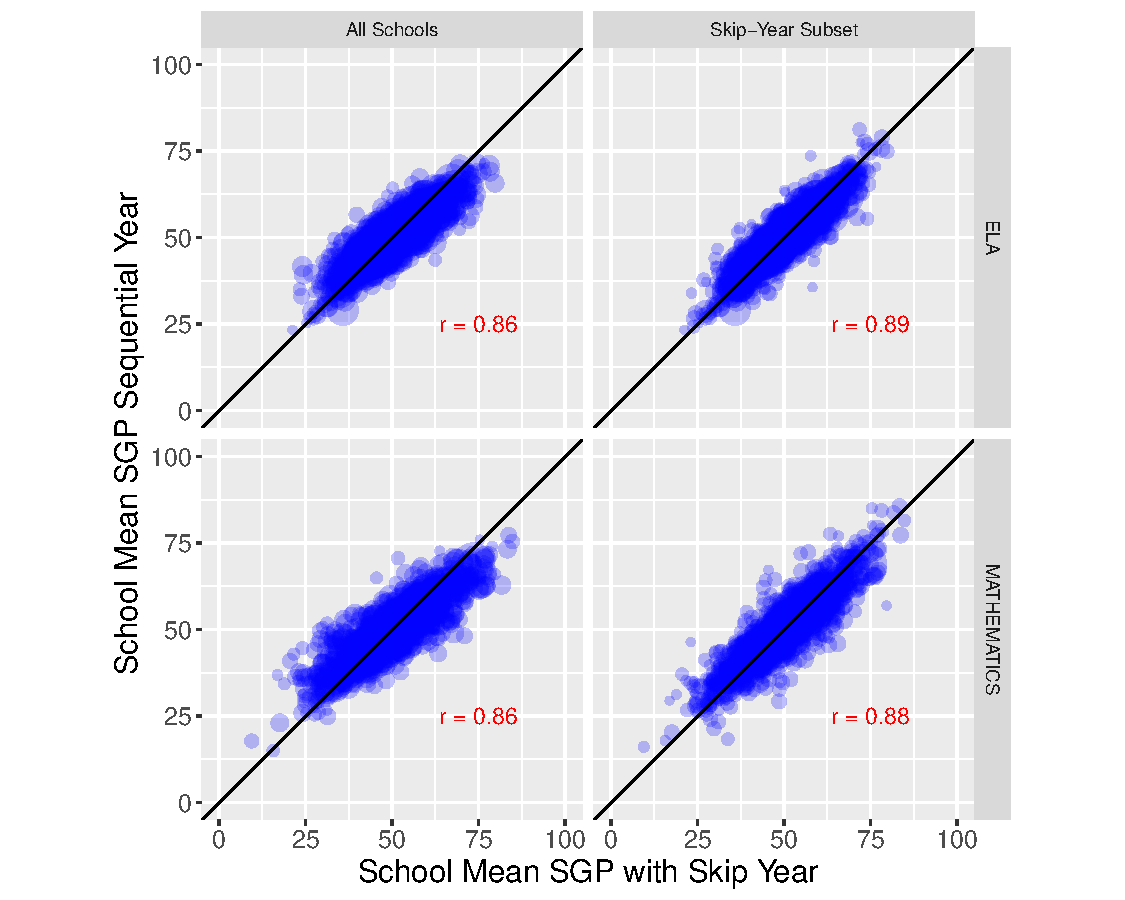
\includegraphics[width=\textwidth]{/Users/avi/Dropbox (SGP)/SGP/State_Alt_Analyses/Demonstration/Skip_Year_Analysis/SGP_Report/assets/img/Skip_Year_SGP_Comp_SGP.pdf}
  \end{subfigure}
\end{figure}

\pagebreak

\hypertarget{school-mean-sgp-differences}{%
\subsubsection{School mean SGP
differences}\label{school-mean-sgp-differences}}

Like at the individual level, a high correlation does not imply the
quantities are identical or interchangeable. Absolute differences
between one-year mean and skip-year mean SGPs were calculated for
schools to provide the average difference for the state by content area.
Table 5 reports these average differences for all students and the
subset of grades for which both skip-year and one-year SGPs were
calculated. On average the differences are small. However, as the
95\(^{th}\) percentile shows, 5 percent of schools report differences in
mean skip-year and one-year SGPs of approximately 14 in Mathematics and
11 in Reading when all students are included. Differences of more than 5
are associated with a small effect size, and are more likely to impact
the accountability sub-indicator ratings that contribute to the larger
school rating. Overall, the differences are middling, neither
insignificant nor egregious.

\begin{table}[H]
\caption*{\textbf{Table 5:} School level skip-year to one-year median and 95th percentile absolute differences\label{table5}} 
\begin{center}
\begin{tabular}{rrcc}
\hline\hline
\multicolumn{1}{c}{Filter}&\multicolumn{1}{c}{Content Area}&\multicolumn{1}{c}{Median Difference}&\multicolumn{1}{c}{95\%ile Difference}\tabularnewline
\hline
&&&\tabularnewline
All Students&Mathematics&5.11&14.36\tabularnewline
&Reading&2.72&11.06\tabularnewline
\hline
&&&\tabularnewline
Skip-Year Subset&Mathematics&5.11&12.13\tabularnewline
&Reading&3.27& 9.08\tabularnewline
\hline
\end{tabular}\end{center}
\end{table}

School size is one driver of the differences in one- and skip-year mean
SGPs to consider. Figure 2 illustrates the relationship between school
level MSGP observed (\emph{not absolute}) differences and school size,
disaggregated by content area and student inclusion filter. In these
plots, MSGP differences are defined as \textbf{skip-year MSGP
\emph{minus} one-year MSGP}; therefore positive numbers can be
interpreted as showing an increase in schools' MSGP when using skip-year
calculations, and vice-versa.

\begin{figure}[H]
\caption*{{{\bf{Figure 2:}} } Mean SGP differences by content area and student inclusion filter}
  \begin{subfigure}[b]{1\textwidth}
    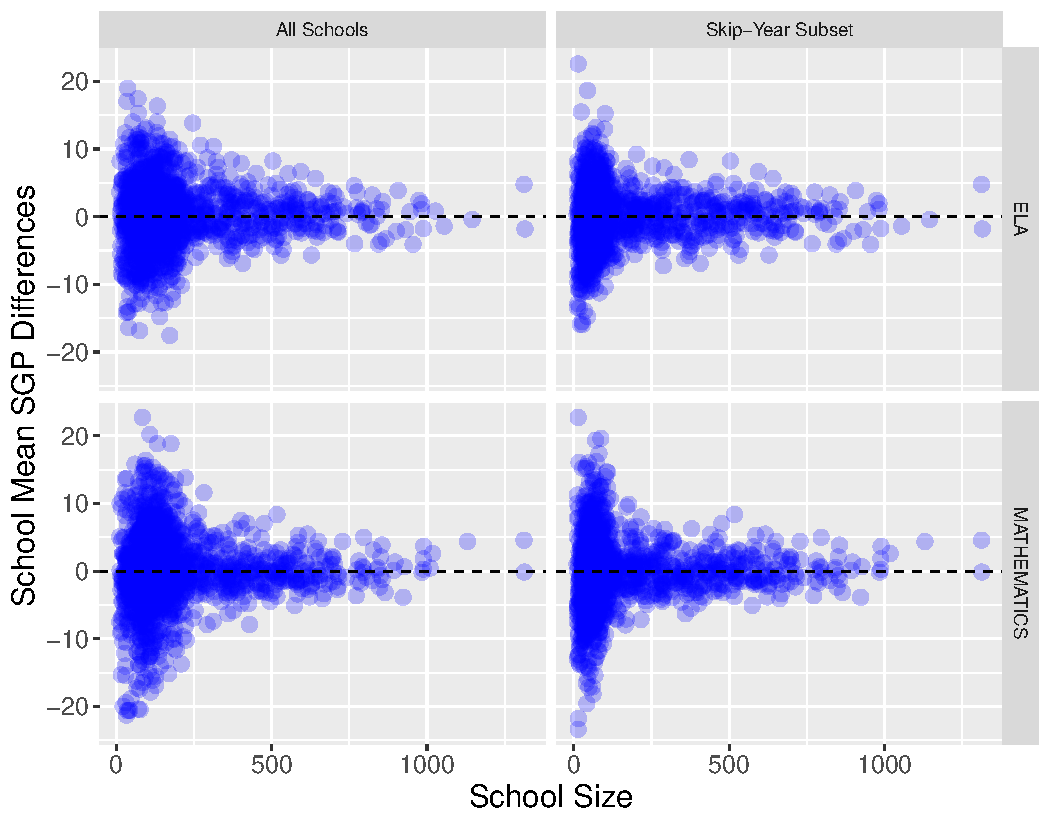
\includegraphics[width=\textwidth]{/Users/avi/Dropbox (SGP)/SGP/State_Alt_Analyses/Demonstration/Skip_Year_Analysis/SGP_Report/assets/img/Skip_Year_SGP_Comp_Diff_x_N.pdf}
  \end{subfigure}
\end{figure}

School level differences like student level differences were, on
average, minor. However, numerous schools showed one-year/skip-year
differences that were not minor and could possibly lead to a different
accountability determination. Further analysis should include re-running
2019 accountability calculations to determine what impact using
skip-year growth in place of one-year growth has on school performance
framework ratings. Such results could be added to this report if made
available or done in cooperation with the Center for Assessment.

\pagebreak

\hypertarget{demographic-subgroup-results}{%
\subsection{Demographic Subgroup
Results}\label{demographic-subgroup-results}}

Issues around opportunity to learn can be investigated using growth gap
comparisons for relevant demographic subgroups. The following
subsections examine differences in the 2019 results for three
demographic groups: economically disadvantaged students (as indicated by
free/reduced-price lunch eligibility status), English language learners,
and students with disabilities (as indicated by having an individualized
education program - IEP). All demographic summaries include only
students who \emph{could} have received a skip-year SGP (i.e.~the
``skip-year subset'') unless otherwise indicated.

Investigations of (differential) impact on student achievement and
growth for already at-risk student populations will be critical to help
ameliorate impacts of the disruption to education from the COVID-19
pandemic.

\hypertarget{economically-disadvantaged-students}{%
\subsubsection{Economically Disadvantaged
Students}\label{economically-disadvantaged-students}}

Table 6 provides the frequencies and proportions of students that had a
sequential and/or skip-year SGP calculated in 2019, disaggregated by
those identified as economically disadvantaged students (eligible for
free/reduced lunch, or FRL), or not, and content area. As the results
show, there is not a considerable difference between the two groups'
growth calculation rates under either analysis.

\begin{table}[H]
\caption*{\textbf{Table 6:} Sequential and skip-year SGP counts and percentages by content area and FRL status\label{table6}} 
\begin{center}
\begin{tabular}{rrrcrrcrr}
\hline\hline
\multicolumn{3}{c}{\bfseries }&\multicolumn{1}{c}{\bfseries }&\multicolumn{2}{c}{\bfseries Sequential}&\multicolumn{1}{c}{\bfseries }&\multicolumn{2}{c}{\bfseries Skip Year}\tabularnewline
\cline{5-6} \cline{8-9}
\multicolumn{1}{c}{Content Area}&\multicolumn{1}{c}{FRL Status}&\multicolumn{1}{c}{Total Students}&\multicolumn{1}{c}{}&\multicolumn{1}{c}{Count}&\multicolumn{1}{c}{Percent}&\multicolumn{1}{c}{}&\multicolumn{1}{c}{Count}&\multicolumn{1}{c}{Percent}\tabularnewline
\hline
&&&&&&&&\tabularnewline
Mathematics&No&19,263&&16,889&87.7&&15,292&79.4\tabularnewline
&Yes&9,038&&7,832&86.7&&7,158&79.2\tabularnewline
\hline
&&&&&&&&\tabularnewline
Reading&No&19,232&&16,848&87.6&&15,235&79.2\tabularnewline
&Yes&9,032&&7,804&86.4&&6,956&77.0\tabularnewline
\hline
\end{tabular}\end{center}
\end{table}

Table 7 provides the correlations between sequential and skip-year SGP
estimates for FRL/non-FRL students that had both a sequential and
skip-year SGP calculated in 2019, as well as the means and standard
deviations for these values. The results show there is not a
considerable difference \emph{within} the two groups' growth under
either analysis. The two growth measures are highly correlated and have
similar distributional qualities within each group by content area.
However, it is important to note the growth gap \emph{between} the
FRL/non-FRL groups in both ELA and Mathematics. This gap is
approximately 7-10 points, on average, for FRL students for the
sequential SGP estimates, and increases to roughly 11-15 points using
the skip-year estimates.

\begin{table}[H]
\caption*{\textbf{Table 7:} Sequential and skip-year SGP correlation and mean/standard deviation by content area and FRL status\label{table7}} 
\begin{center}
\begin{tabular}{rrccccccc}
\hline\hline
\multicolumn{3}{c}{\bfseries }&\multicolumn{1}{c}{\bfseries }&\multicolumn{2}{c}{\bfseries Sequential}&\multicolumn{1}{c}{\bfseries }&\multicolumn{2}{c}{\bfseries Skip Year}\tabularnewline
\cline{5-6} \cline{8-9}
\multicolumn{1}{c}{Content Area}&\multicolumn{1}{c}{FRL Status}&\multicolumn{1}{c}{SGP Correlation}&\multicolumn{1}{c}{}&\multicolumn{1}{c}{Mean}&\multicolumn{1}{c}{SD}&\multicolumn{1}{c}{}&\multicolumn{1}{c}{Mean}&\multicolumn{1}{c}{SD}\tabularnewline
\hline
&&&&&&&&\tabularnewline
Mathematics&No&0.76&&53.0&28.6&&54.7&28.1\tabularnewline
&Yes&0.77&&43.4&28.4&&40.1&28.1\tabularnewline
\hline
&&&&&&&&\tabularnewline
Reading&No&0.83&&51.9&28.7&&53.5&28.4\tabularnewline
&Yes&0.82&&44.8&28.7&&42.4&28.3\tabularnewline
\hline
\end{tabular}\end{center}
\end{table}

Table 8 provides the correlations between school level sequential and
skip-year MSGP estimates and the schools' percentage of FRL students. As
with the school level summary results in the previous section, these
summaries are provided for both 1) all students (including 4\(^{th}\)
graders) and 2) for the subset of students that have both a sequential
and skip-year SGP calculated in 2019. The results show a negative
relationship (correlation) between typical school growth and the school
percentage of FRL students. That is, the schools with larger FRL
populations tend to demonstrate lower academic growth.

\begin{table}[H]
\caption*{\textbf{Table 8:} School level correlations between mean SGPs and percent FRL by student inclusion filter\label{table8}} 
\begin{center}
\begin{tabular}{rrrr}
\hline\hline
\multicolumn{1}{c}{Filter}&\multicolumn{1}{c}{Content Area}&\multicolumn{1}{c}{Sequential}&\multicolumn{1}{c}{Skip Year}\tabularnewline
\hline
&&&\tabularnewline
All Students&Mathematics&-0.54&-0.62\tabularnewline
&Reading&-0.57&-0.69\tabularnewline
\hline
&&&\tabularnewline
Skip-Year Subset&Mathematics&-0.58&-0.63\tabularnewline
&Reading&-0.51&-0.69\tabularnewline
\hline
\end{tabular}\end{center}
\end{table}

Figure 3 is a visual representation of school level MSGP differences as
a function of school FRL population size by content area and student
inclusion filter. MSGP differences are defined as \textbf{skip-year MSGP
\emph{minus} one-year MSGP}, and therefore positive numbers can be
interpreted as showing an increase in schools' MSGP when using skip-year
calculations, and vice-versa. Bubble sizes are representative of school
size, and the black line is a LOESS smoothing curve that depicts the
moving average MSGP difference relative to the percent FRL.

This plot shows a slight negative relationship between the MSGP
difference and FRL population size. This suggests that, on average,
schools with higher FRL populations have lower difference values
(i.e.~schools with larger FRL populations may be slightly more likely to
be negatively impacted with the use of skip-year analysis).

\begin{figure}[H]
\caption*{{{\bf{Figure 3:}} } Mean SGP difference by percent FRL by content area and student inclusion filter}
  \begin{subfigure}[b]{1\textwidth}
    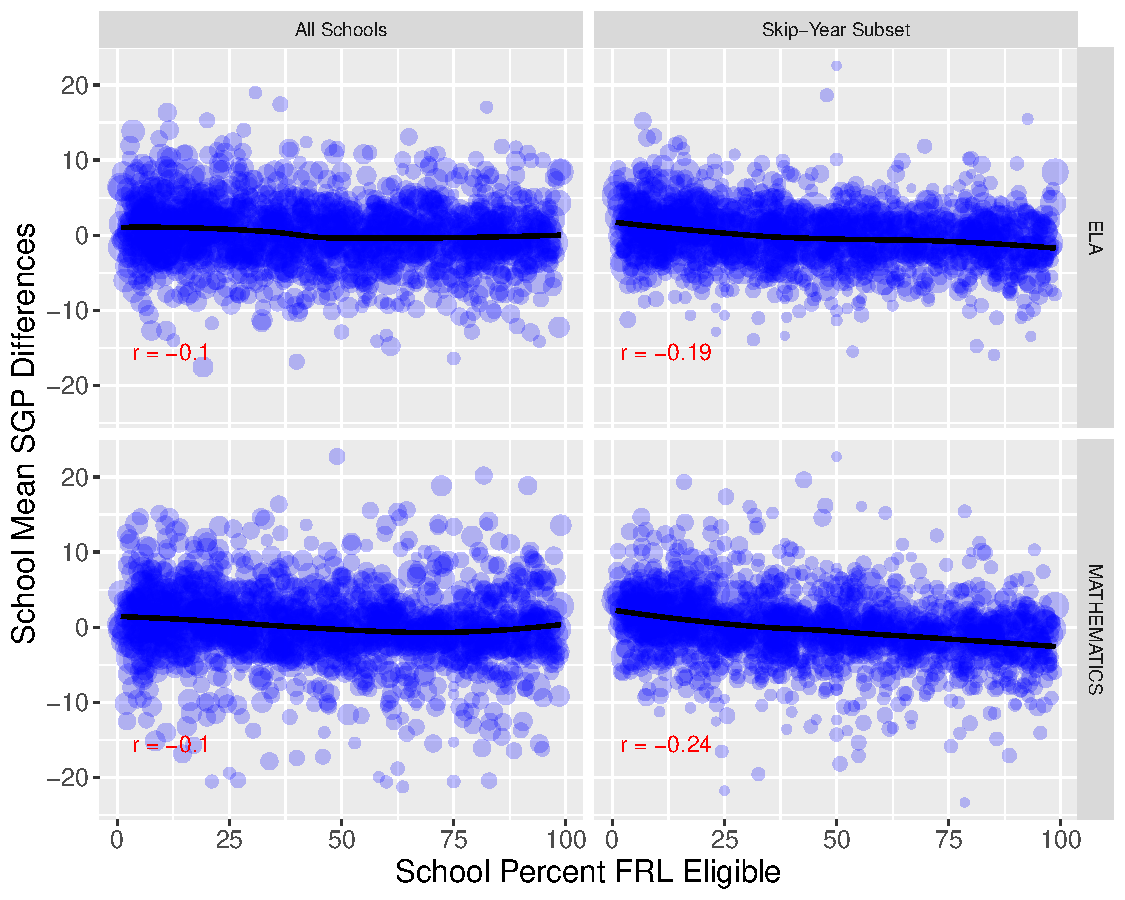
\includegraphics[width=\textwidth]{/Users/avi/Dropbox (SGP)/SGP/State_Alt_Analyses/Demonstration/Skip_Year_Analysis/SGP_Report/assets/img/Skip_Year_SGP_Comp_SGP_x_FRL.pdf}
  \end{subfigure}
\end{figure}

\hypertarget{english-language-learners}{%
\subsubsection{English Language
Learners}\label{english-language-learners}}

Table 9 provides the frequencies and proportions of students that had a
sequential and/or skip-year SGP calculated in 2019, disaggregated by
those identified as English language learners (ELL), or not, and content
area. As the results show, there is not a considerable difference
between the two groups' growth calculation rates under either analysis.
However, roughly 10\% fewer students receive a SGP calculation under the
skip-year approach.

\begin{table}[H]
\caption*{\textbf{Table 9:} Sequential and skip-year SGP counts and percentages by content area and ELL status\label{table9}} 
\begin{center}
\begin{tabular}{rrrcrrcrr}
\hline\hline
\multicolumn{3}{c}{\bfseries }&\multicolumn{1}{c}{\bfseries }&\multicolumn{2}{c}{\bfseries Sequential}&\multicolumn{1}{c}{\bfseries }&\multicolumn{2}{c}{\bfseries Skip Year}\tabularnewline
\cline{5-6} \cline{8-9}
\multicolumn{1}{c}{Content Area}&\multicolumn{1}{c}{ELL Status}&\multicolumn{1}{c}{Total Students}&\multicolumn{1}{c}{}&\multicolumn{1}{c}{Count}&\multicolumn{1}{c}{Percent}&\multicolumn{1}{c}{}&\multicolumn{1}{c}{Count}&\multicolumn{1}{c}{Percent}\tabularnewline
\hline
&&&&&&&&\tabularnewline
Mathematics&No&25,341&&22,061&87.1&&19,968&78.8\tabularnewline
&Yes&2,960&&2,660&89.9&&2,482&83.9\tabularnewline
\hline
&&&&&&&&\tabularnewline
Reading&No&25,316&&22,015&87.0&&19,916&78.7\tabularnewline
&Yes&2,948&&2,637&89.5&&2,275&77.2\tabularnewline
\hline
\end{tabular}\end{center}
\end{table}

Table 10 provides the correlations between sequential and skip-year SGP
estimates for ELL/non-ELL students that had both a sequential and
skip-year SGP calculated in 2019, as well as the means and standard
deviations for these values. The two growth measures are highly
correlated and have similar distributional qualities within each group
by content area. There is a slight difference \emph{within} the ELL
group's growth calculation between the sequential and skip-year
analyses. This results in increasing the otherwise modest growth gap
between ELL and non-ELL students in Mathematics between the sequential
and skip-year analyses.

\begin{table}[H]
\caption*{\textbf{Table 10:} Sequential and skip-year SGP correlation and mean/standard deviation by content area and ELL status\label{table10}} 
\begin{center}
\begin{tabular}{rrccccccc}
\hline\hline
\multicolumn{3}{c}{\bfseries }&\multicolumn{1}{c}{\bfseries }&\multicolumn{2}{c}{\bfseries Sequential}&\multicolumn{1}{c}{\bfseries }&\multicolumn{2}{c}{\bfseries Skip Year}\tabularnewline
\cline{5-6} \cline{8-9}
\multicolumn{1}{c}{Content Area}&\multicolumn{1}{c}{ELL Status}&\multicolumn{1}{c}{SGP Correlation}&\multicolumn{1}{c}{}&\multicolumn{1}{c}{Mean}&\multicolumn{1}{c}{SD}&\multicolumn{1}{c}{}&\multicolumn{1}{c}{Mean}&\multicolumn{1}{c}{SD}\tabularnewline
\hline
&&&&&&&&\tabularnewline
Mathematics&No&0.77&&50.3&28.9&&50.5&28.8\tabularnewline
&Yes&0.79&&47.2&28.9&&46.3&29.3\tabularnewline
\hline
&&&&&&&&\tabularnewline
Reading&No&0.83&&49.6&29.0&&50.1&28.9\tabularnewline
&Yes&0.84&&50.3&28.3&&49.2&28.7\tabularnewline
\hline
\end{tabular}\end{center}
\end{table}

Table 11 provides the correlations between school level sequential and
skip-year MSGP estimates and the schools' percentage of ELL students. As
with the school level summary results in the previous section, these
summaries are provided for both 1) all students (including 4\(^{th}\)
graders) and 2) for the subset of students that have both a sequential
and skip-year SGP calculated in 2019. As the results show, the
relationship (correlation) between mean growth and the school percentage
of ELL students is moderately negative.

\begin{table}[H]
\caption*{\textbf{Table 11:} School level correlations between mean SGPs and percent ELL by student inclusion filter\label{table11}} 
\begin{center}
\begin{tabular}{rrrr}
\hline\hline
\multicolumn{1}{c}{Filter}&\multicolumn{1}{c}{Content Area}&\multicolumn{1}{c}{Sequential}&\multicolumn{1}{c}{Skip Year}\tabularnewline
\hline
&&&\tabularnewline
All Students&Mathematics&-0.23&-0.12\tabularnewline
&Reading&-0.18&-0.18\tabularnewline
\hline
&&&\tabularnewline
Skip-Year Subset&Mathematics&-0.17&-0.15\tabularnewline
&Reading&-0.07&-0.15\tabularnewline
\hline
\end{tabular}\end{center}
\end{table}

Figure 4 is a visual representation of school level MSGP differences as
a function of school ELL population size by content area and student
inclusion filter. MSGP differences are defined as \textbf{skip-year MSGP
\emph{minus} one-year MSGP}, and therefore positive numbers can be
interpreted as showing an increase in schools' MSGP when using skip-year
calculations, and vice-versa. Bubble sizes are representative of school
size, and the black line is a LOESS smoothing curve that depicts the
moving average MSGP difference relative to the percent ELL.

This plot shows a slightly negative relationship between the MSGP
difference and ELL population size for the skip-year subset,
particularly in Reading. This suggests that, on average, schools with
higher ELL populations have lower difference values in Reading
(i.e.~schools with larger ELL populations are slightly more likely to be
negatively impacted with the use of skip-year analysis, although this
impact appears to modest).

\begin{figure}[H]
\caption*{{{\bf{Figure 4:}} } Mean SGP difference by percent ELL by content area and student inclusion filter}
  \begin{subfigure}[b]{1\textwidth}
    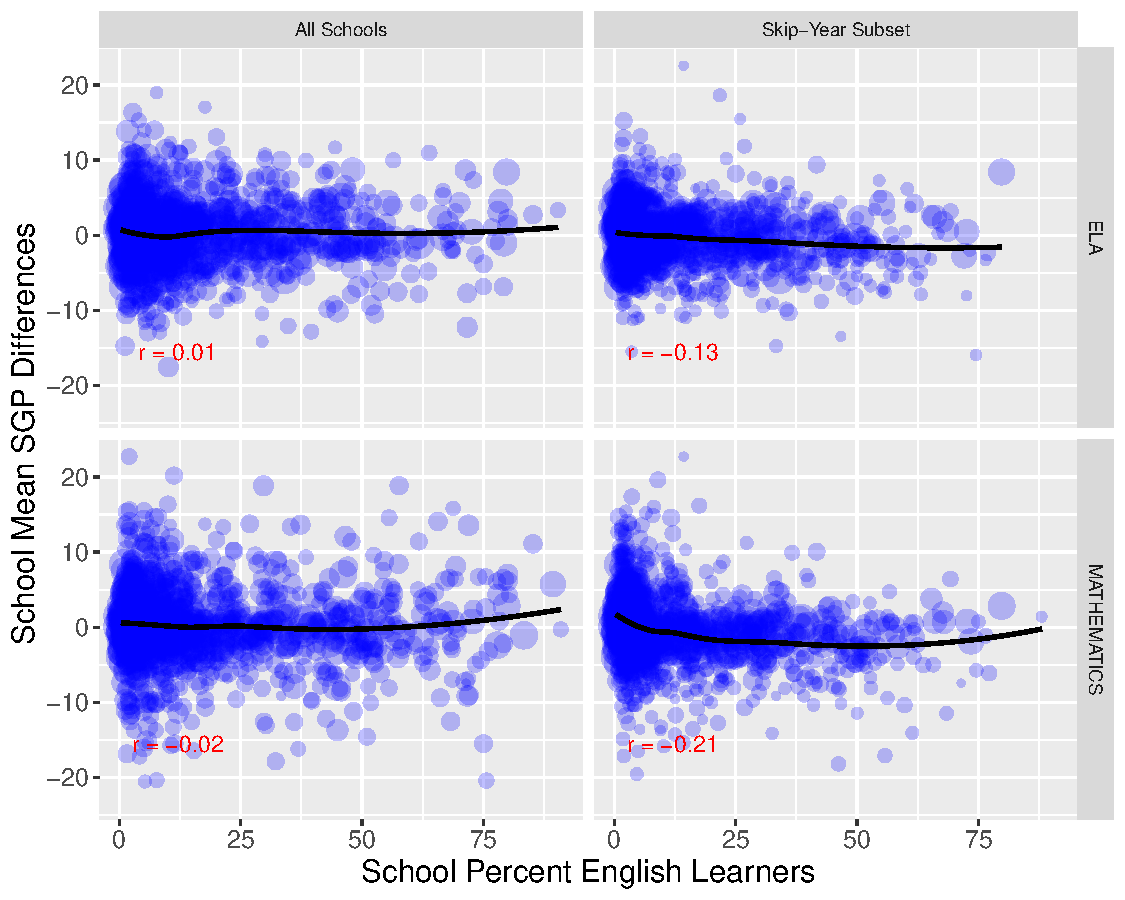
\includegraphics[width=\textwidth]{/Users/avi/Dropbox (SGP)/SGP/State_Alt_Analyses/Demonstration/Skip_Year_Analysis/SGP_Report/assets/img/Skip_Year_SGP_Comp_SGP_x_ELL.pdf}
  \end{subfigure}
\end{figure}

\hypertarget{students-with-disabilities}{%
\subsubsection{Students with
Disabilities}\label{students-with-disabilities}}

Table 12 provides the frequencies and proportions of students that had a
sequential and/or skip-year SGP calculated in 2019, disaggregated by
those identified as students with disabilities (or SWD, indicated as
having an IEP), or not, and content area. As the results show, there is
not a considerable difference between the two groups' growth calculation
rates under either analysis, although students with disabilities (SWD)
do receive SGP estimates at slightly lower rate than those without.

\begin{table}[H]
\caption*{\textbf{Table 12:} Sequential and skip-year SGP counts and percentages by content area and SWD status\label{table12}} 
\begin{center}
\begin{tabular}{rrrcrrcrr}
\hline\hline
\multicolumn{3}{c}{\bfseries }&\multicolumn{1}{c}{\bfseries }&\multicolumn{2}{c}{\bfseries Sequential}&\multicolumn{1}{c}{\bfseries }&\multicolumn{2}{c}{\bfseries Skip Year}\tabularnewline
\cline{5-6} \cline{8-9}
\multicolumn{1}{c}{Content Area}&\multicolumn{1}{c}{SWD Status}&\multicolumn{1}{c}{Total Students}&\multicolumn{1}{c}{}&\multicolumn{1}{c}{Count}&\multicolumn{1}{c}{Percent}&\multicolumn{1}{c}{}&\multicolumn{1}{c}{Count}&\multicolumn{1}{c}{Percent}\tabularnewline
\hline
&&&&&&&&\tabularnewline
Mathematics&No&26,348&&23,077&87.6&&20,968&79.6\tabularnewline
&Yes&1,953&&1,644&84.2&&1,482&75.9\tabularnewline
\hline
&&&&&&&&\tabularnewline
Reading&No&26,301&&23,014&87.5&&20,728&78.8\tabularnewline
&Yes&1,963&&1,638&83.4&&1,463&74.5\tabularnewline
\hline
\end{tabular}\end{center}
\end{table}

Table 13 provides the correlations between sequential and skip-year SGP
estimates for SWD/non-SWD students that had both a sequential and
skip-year SGP calculated in 2019, as well as the means and standard
deviations for these values. The results show that the two growth
measures are highly correlated and have similar distributional qualities
within each group by content area. There is a slight difference
\emph{within} the SWD group's MSGPs between the sequential and skip-year
analyses. Specifically, this group's typical growth in both ELA and
Mathematics are 1-3 points lower using the skip-year analysis, thus
increasing the existing growth gap between SWD and non-SWD populations.
The gap is 7 points, on average, for the sequential SGP estimates, and
increases slightly to approximately 9 points using the skip-year
estimates.

\begin{table}[H]
\caption*{\textbf{Table 13:} Sequential and skip-year SGP correlation and mean/standard deviation by content area and SWD status\label{table13}} 
\begin{center}
\begin{tabular}{rrccccccc}
\hline\hline
\multicolumn{3}{c}{\bfseries }&\multicolumn{1}{c}{\bfseries }&\multicolumn{2}{c}{\bfseries Sequential}&\multicolumn{1}{c}{\bfseries }&\multicolumn{2}{c}{\bfseries Skip Year}\tabularnewline
\cline{5-6} \cline{8-9}
\multicolumn{1}{c}{Content Area}&\multicolumn{1}{c}{SWD Status}&\multicolumn{1}{c}{SGP Correlation}&\multicolumn{1}{c}{}&\multicolumn{1}{c}{Mean}&\multicolumn{1}{c}{SD}&\multicolumn{1}{c}{}&\multicolumn{1}{c}{Mean}&\multicolumn{1}{c}{SD}\tabularnewline
\hline
&&&&&&&&\tabularnewline
Mathematics&No&0.77&&50.4&28.8&&50.6&28.8\tabularnewline
&Yes&0.81&&44.2&29.9&&41.5&29.8\tabularnewline
\hline
&&&&&&&&\tabularnewline
Reading&No&0.83&&50.2&28.8&&50.6&28.7\tabularnewline
&Yes&0.80&&42.6&29.0&&41.3&29.2\tabularnewline
\hline
\end{tabular}\end{center}
\end{table}

Table 14 provides the correlations between school level sequential and
skip-year MSGP estimates and the schools' percentage of SWD students. As
with the school level summary results in the previous section, these
summaries are provided for both 1) all students (including 4\(^{th}\)
graders) and 2) for the subset of students that have both a sequential
and skip-year SGP calculated in 2019. As the results show, a negative
relationship (correlation) exists between typical school growth and the
school SWD percentage. That is, the schools with larger populations of
students with disabilities tend to demonstrate lower academic growth.

\begin{table}[H]
\caption*{\textbf{Table 14:} School level correlations between mean SGPs and percent SWD by student inclusion filter\label{table14}} 
\begin{center}
\begin{tabular}{rrrr}
\hline\hline
\multicolumn{1}{c}{Filter}&\multicolumn{1}{c}{Content Area}&\multicolumn{1}{c}{Sequential}&\multicolumn{1}{c}{Skip Year}\tabularnewline
\hline
&&&\tabularnewline
All Students&Mathematics&-0.32&-0.29\tabularnewline
&Reading&-0.32&-0.35\tabularnewline
\hline
&&&\tabularnewline
Skip-Year Subset&Mathematics&-0.37&-0.40\tabularnewline
&Reading&-0.41&-0.48\tabularnewline
\hline
\end{tabular}\end{center}
\end{table}

Figure 5 is a visual representation of school level MSGP differences as
a function of school SWD population size by content area and student
inclusion filter. MSGP differences are defined as \textbf{skip-year MSGP
\emph{minus} one-year MSGP}, and therefore positive numbers can be
interpreted as showing an increase in schools' MSGP when using skip-year
calculations, and vice-versa. Bubble sizes are representative of school
size, and the black line is a LOESS smoothing curve that depicts the
moving average MSGP difference relative to the percent SWD.

The plots show slight negative relationships between MSGP difference and
SWD population size for the skip-year subset. This suggests that, on
average, schools with higher SWD populations have lower difference
values (i.e.~schools with larger SWD populations are slightly more
likely to be negatively impacted with the use of skip-year analysis).
Note that the range of school percent SWD is restricted to 0 to 25\%.

\begin{figure}[H]
\caption*{{{\bf{Figure 5:}} } Mean SGP difference by percent SWD by content area and student inclusion filter}
  \begin{subfigure}[b]{1\textwidth}
    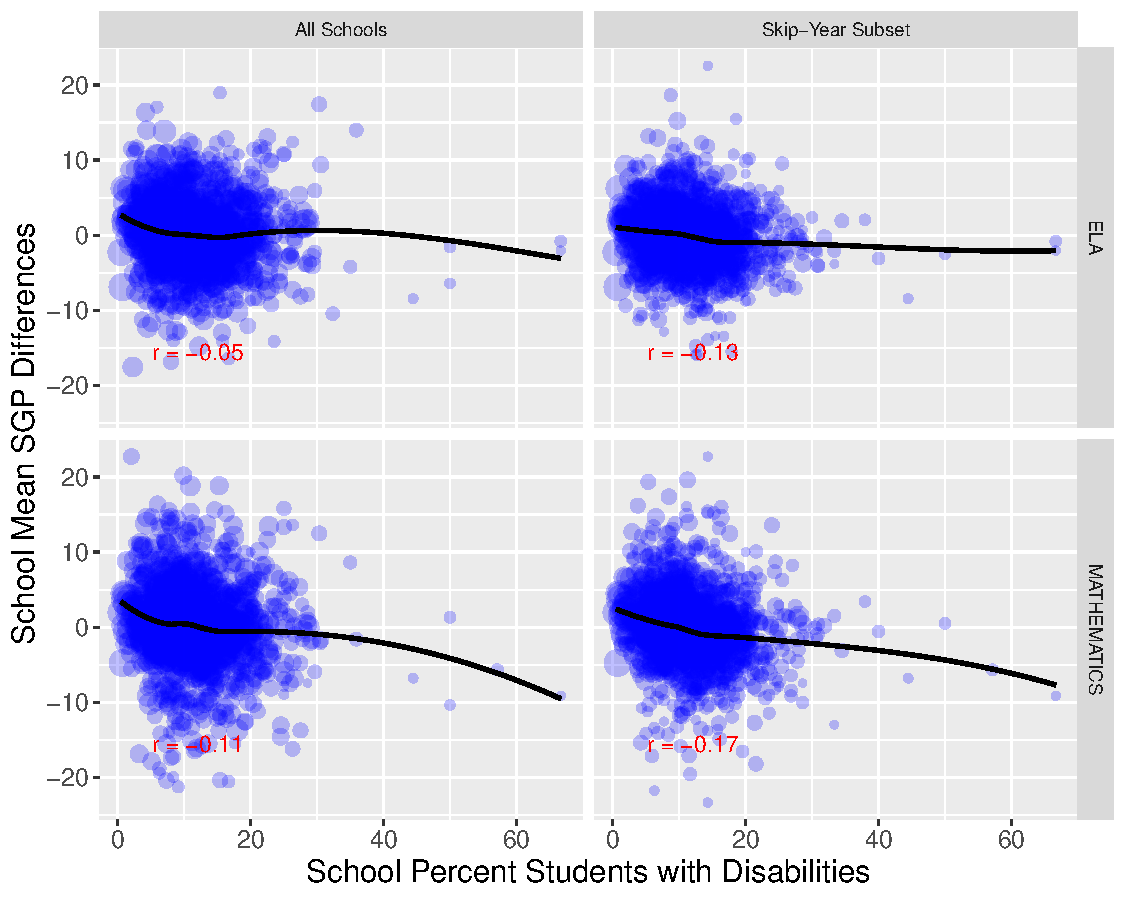
\includegraphics[width=\textwidth]{/Users/avi/Dropbox (SGP)/SGP/State_Alt_Analyses/Demonstration/Skip_Year_Analysis/SGP_Report/assets/img/Skip_Year_SGP_Comp_SGP_x_SWD.pdf}
  \end{subfigure}
\end{figure}

\pagebreak

\hypertarget{summary}{%
\section{Summary}\label{summary}}

The analyses conducted in this report investigate whether skip-year SGPs
can be used in place of the standard one-year SGPs. The report discussed
four potential issues:

\begin{itemize}
\tightlist
\item
  Are the students with skip-year SGPs systematically different than
  those with one-year SGPs?
\item
  Are the one-year SGPs systematically different than the skip-year SGPs
  at the individual level?
\item
  Are the one-year SGPs systematically different than the skip-year SGPs
  when aggregated to the school level?
\item
  Are the one-year SGPs systematically different than the skip-year SGPs
  for different demographic subgroups?
\end{itemize}

\noindent No significant systematic differences were found for any of
these questions. This is not to say there were not differences worth
considering for a minority of students and schools. The results produced
by these analyses do not disqualify the use of skip-year growth in lieu
of one-year growth. However, they do not unequivocally qualify their use
either. Since the results here are generated from historical data
derived under ``usual'' educational circumstances and the current
circumstances are far from usual, it is likely that spring 2021
skip-year data will exhibit greater deviations than what is reported
here. Until confirmation is available that 2021 skip-year deviations are
no larger than they were historically, it is not possible to assure the
usability of skip-year growth for business-as-usual accountability.

Beyond the technical characteristics of skip-year growth lie numerous
practical and political considerations for its use in both state and
federal accountability. As Demonstration approaches 2021, any decisions
related to student testing and accountability will require some
technical consideration, but much more practical and political
calculation to determine the best course of action going forward.

Assuming testing does occur in some form in 2021, it is highly
recommended that growth be calculated regardless of whether it is used
for accountability. There are numerous, valuable inquiries that can be
addressed with skip-year SGPs available including:

\begin{itemize}
\tightlist
\item
  What was the overall impact on student learning in the state of
  Demonstration due to COVID-19?
\item
  What demographic subgroups fared best and which demographic subgroups
  fared most poorly in terms of learning during the COVID-19 pandemic?
\item
  Are there COVID-19 related instructional approaches that led to
  greater student learning than others? If so, what were they and how
  much more learning were they associated with?
\end{itemize}

\noindent Critical to the investigation of COVID-19 related learning
loss will be accurate data on COVID-19 related education programs and
student participation over time. Collecting these data would allow the
Student Growth Percentiles Package to leverage student growth data and
inform stakeholders about the impacts of the COVID-19 pandemic on
student educational outcomes.

\pagebreak

\hypertarget{references}{%
\section*{References}\label{references}}
\addcontentsline{toc}{section}{References}

\hypertarget{refs}{}
\begin{cslreferences}
\leavevmode\hypertarget{ref-sgp2020}{}%
Betebenner, D. W., VanIwaarden, A., Domingue, B., \& Shang, Y. (2020).
\emph{SGP: Student growth percentiles \& percentile growth
trajectories.} Retrieved from \url{sgp.io}

\leavevmode\hypertarget{ref-Rsoftware}{}%
R Core Team. (2020). \emph{{{R}}: A language and environment for
statistical computing}. Vienna, Austria: R Foundation for Statistical
Computing. Retrieved from \url{http://www.R-project.org}
\end{cslreferences}

\pagebreak

\renewcommand{\thesection}{A}
\titleformat{\section}{\normalfont\Large\bfseries}{}{0pt}{}
\pagenumbering{arabic}
\renewcommand*{\thepage}{\thesection\arabic{page}}

\hypertarget{appendices}{%
\section{Appendix A - Goodness of Fit Plots}\label{appendices}}

A goodness of fit plot is produced for each unique analysis run in 2019.
All fit plots will contain at least four panels. Each panel is a
different depiction of the distribution of the Student Growth
Percentiles (SGPs) calculated in that analysis relative to the students'
prior or current achievement (i.e.~the test scores used as the
independent and dependent variables in the model).

The top panel is a mosaic plot that shows the percentage of students
that fall into each prior proficiency level, and the location of the
10\(^{th}\) through 90\(^{th}\) deciles of the SGP distribution
represented as dashed white lines (with the exception of the solid white
line for the median/50\(^{th}\) percentile). Ideally the median SGP will
be at or near 50 for all prior achievement level groups. The top panel
is excluded when students' prior achievement level data is unavailable.

The ``Ceiling/Floor Effects Test'' panel helps identify problems in SGP
estimation at the Highest and Lowest Obtainable/Observed Scale Scores
(HOSS and LOSS). The table of values shows whether the current year
scores at both extremes yield expected SGP values. The expectation is
that the majority of SGPs for students scoring at or near the LOSS will
be low (preferably less than 5 and not higher than 20), and that SGPs
for students scoring at or near the HOSS will be high (preferably higher
than 95 and not less than 80). Because few students may score
\emph{exactly} at the HOSS/LOSS, the top/bottom 50 students are selected
and any student scoring within their range of scores are selected for
inclusion in these tables. Consequently, there may be a range of scores
at the HOSS/LOSS rather than a single score, and there may be more than
50 students included in the HOSS/LOSS row if the 50 students at the
extremes only contain the single HOSS/LOSS score.

The ``Student Growth Percentile Range'' panel at bottom left shows the
empirical distribution of SGPs given prior scale score deciles in the
form of a 10 by 10 cell grid. Percentages of student growth percentiles
between the 10\(^{th}\), 20\(^{th}\), 30\(^{th}\), 40\(^{th}\),
50\(^{th}\), 60\(^{th}\), 70\(^{th}\), 80\(^{th}\), and 90\(^{th}\)
percentiles were calculated based upon the empirical decile of the
cohort's prior year scaled score distribution\footnote{The total
  students in each analysis varies depending on grade and subject, and
  prior score deciles are based only on scores for students used in the
  SGP calculations.}. Deviations from perfect fit are indicated by red
and blue shading. The further above 10 the darker the red, and the
further below 10 the darker the blue.

The bottom right panel of each plot is a
\href{https://en.wikipedia.org/wiki/Q\%E2\%80\%93Q_plot}{Q-Q plot} which
compares the observed distribution of SGPs with the theoretical
(uniform) distribution. An ideal plot here will show black step function
lines that do not deviate from the ideal, red line which traces the 45
degree angle of perfect fit.

The following sections provide the fit plots for the sequential and skip
year analyses. The first section provides the 4\(^{th}\) grade
Mathematics and Reading plots for the 2019 sequential analyses only.
These provide context for what a single prior one-year analysis looks
like for Demonstration. The subsequent sections provides the fit plots
from both sequential and skip-year analyses for Mathematics And Reading.
In these two content area specific sections, the grade level analysis
plots are presented with each grade in a row; sequential analyses are in
the left column and skip-year analyses are in the right column.

\hypertarget{sequential-analyses-only}{%
\subsection{Sequential Analyses Only}\label{sequential-analyses-only}}

\begin{figure}[H]
\caption*{{{\bf{Figure A1:}} } Sequential growth goodness of fit plots for 4$^{th}$ grade Mathematics and Reading (no skip-year analyses)}
  \begin{subfigure}[b]{0.5\textwidth}
    \includegraphics[width=\textwidth]{/Users/avi/Dropbox (SGP)/SGP/State_Alt_Analyses/Demonstration/Skip_Year_Analysis/Sequential_GOF/Goodness_of_Fit/MATHEMATICS.2018_2019/2018_2019_MATH_4;2017_2018_MATH_3.pdf}
  \end{subfigure}
  \begin{subfigure}[b]{0.5\textwidth}
    \includegraphics[width=\textwidth]{/Users/avi/Dropbox (SGP)/SGP/State_Alt_Analyses/Demonstration/Skip_Year_Analysis/Sequential_GOF/Goodness_of_Fit/READING.2018_2019/2018_2019_READING_4;2017_2018_READING_3.pdf}
  \end{subfigure}
\end{figure}

\hypertarget{mathematics}{%
\subsection{Mathematics}\label{mathematics}}

\begin{figure}[H]
\caption*{{{\bf{Figure A2:}} } Sequential (left) and skip-year (right) fit plots for Math (grades 5 - 6)}
  \begin{subfigure}[b]{0.5\textwidth}
    \includegraphics[width=\textwidth]{/Users/avi/Dropbox (SGP)/SGP/State_Alt_Analyses/Demonstration/Skip_Year_Analysis/Sequential_GOF/Goodness_of_Fit/MATHEMATICS.2018_2019/2018_2019_MATH_5;2017_2018_MATH_4;2016_2017_MATH_3.pdf}
  \end{subfigure}
  \begin{subfigure}[b]{0.5\textwidth}
    \includegraphics[width=\textwidth]{/Users/avi/Dropbox (SGP)/SGP/State_Alt_Analyses/Demonstration/Skip_Year_Analysis/Goodness_of_Fit/MATHEMATICS.2018_2019/2018_2019_MATH_5;2016_2017_MATH_3.pdf}
  \end{subfigure}
  \begin{subfigure}[b]{0.5\textwidth}
    \includegraphics[width=\textwidth]{/Users/avi/Dropbox (SGP)/SGP/State_Alt_Analyses/Demonstration/Skip_Year_Analysis/Sequential_GOF/Goodness_of_Fit/MATHEMATICS.2018_2019/2018_2019_MATH_6;2017_2018_MATH_5;2016_2017_MATH_4;2015_2016_MATH_3.pdf}
  \end{subfigure}
  \begin{subfigure}[b]{0.5\textwidth}
    \includegraphics[width=\textwidth]{/Users/avi/Dropbox (SGP)/SGP/State_Alt_Analyses/Demonstration/Skip_Year_Analysis/Goodness_of_Fit/MATHEMATICS.2018_2019/2018_2019_MATH_6;2016_2017_MATH_4;2015_2016_MATH_3.pdf}
  \end{subfigure}
\end{figure}

\begin{figure}[H]
\caption*{{{\bf{Figure A3:}} } Sequential (left) and skip-year (right) fit plots for Math (grades 7 - 8)}
  \begin{subfigure}[b]{0.5\textwidth}
    \includegraphics[width=\textwidth]{/Users/avi/Dropbox (SGP)/SGP/State_Alt_Analyses/Demonstration/Skip_Year_Analysis/Sequential_GOF/Goodness_of_Fit/MATHEMATICS.2018_2019/2018_2019_MATH_7;2017_2018_MATH_6;2016_2017_MATH_5;2015_2016_MATH_4.pdf}
  \end{subfigure}
  \begin{subfigure}[b]{0.5\textwidth}
    \includegraphics[width=\textwidth]{/Users/avi/Dropbox (SGP)/SGP/State_Alt_Analyses/Demonstration/Skip_Year_Analysis/Goodness_of_Fit/MATHEMATICS.2018_2019/2018_2019_MATH_7;2016_2017_MATH_5;2015_2016_MATH_4.pdf}
  \end{subfigure}
  \begin{subfigure}[b]{0.5\textwidth}
    \includegraphics[width=\textwidth]{/Users/avi/Dropbox (SGP)/SGP/State_Alt_Analyses/Demonstration/Skip_Year_Analysis/Sequential_GOF/Goodness_of_Fit/MATHEMATICS.2018_2019/2018_2019_MATH_8;2017_2018_MATH_7;2016_2017_MATH_6;2015_2016_MATH_5.pdf}
  \end{subfigure}
  \begin{subfigure}[b]{0.5\textwidth}
    \includegraphics[width=\textwidth]{/Users/avi/Dropbox (SGP)/SGP/State_Alt_Analyses/Demonstration/Skip_Year_Analysis/Goodness_of_Fit/MATHEMATICS.2018_2019/2018_2019_MATH_8;2016_2017_MATH_6;2015_2016_MATH_5.pdf}
  \end{subfigure}
\end{figure}

\begin{figure}[H]
\caption*{{{\bf{Figure A4:}} } Sequential (left) and skip-year (right) fit plots for Math (grades 9 - 10)}
  \begin{subfigure}[b]{0.5\textwidth}
    \includegraphics[width=\textwidth]{/Users/avi/Dropbox (SGP)/SGP/State_Alt_Analyses/Demonstration/Skip_Year_Analysis/Sequential_GOF/Goodness_of_Fit/MATHEMATICS.2018_2019/2018_2019_MATH_9;2017_2018_MATH_8;2016_2017_MATH_7;2015_2016_MATH_6.pdf}
  \end{subfigure}
  \begin{subfigure}[b]{0.5\textwidth}
    \includegraphics[width=\textwidth]{/Users/avi/Dropbox (SGP)/SGP/State_Alt_Analyses/Demonstration/Skip_Year_Analysis/Goodness_of_Fit/MATHEMATICS.2018_2019/2018_2019_MATH_9;2016_2017_MATH_7;2015_2016_MATH_6.pdf}
  \end{subfigure}
  \begin{subfigure}[b]{0.5\textwidth}
    \includegraphics[width=\textwidth]{/Users/avi/Dropbox (SGP)/SGP/State_Alt_Analyses/Demonstration/Skip_Year_Analysis/Sequential_GOF/Goodness_of_Fit/MATHEMATICS.2018_2019/2018_2019_MATH_10;2017_2018_MATH_9;2016_2017_MATH_8;2015_2016_MATH_7.pdf}
  \end{subfigure}
  \begin{subfigure}[b]{0.5\textwidth}
    \includegraphics[width=\textwidth]{/Users/avi/Dropbox (SGP)/SGP/State_Alt_Analyses/Demonstration/Skip_Year_Analysis/Goodness_of_Fit/MATHEMATICS.2018_2019/2018_2019_MATH_10;2016_2017_MATH_8;2015_2016_MATH_7.pdf}
  \end{subfigure}
\end{figure}

\hypertarget{reading}{%
\subsection{Reading}\label{reading}}

\begin{figure}[H]
\caption*{{{\bf{Figure A5:}} } Sequential (left) and skip-year (right) fit plots for Reading (grades 5 - 6)}
  \begin{subfigure}[b]{0.5\textwidth}
    \includegraphics[width=\textwidth]{/Users/avi/Dropbox (SGP)/SGP/State_Alt_Analyses/Demonstration/Skip_Year_Analysis/Sequential_GOF/Goodness_of_Fit/READING.2018_2019/2018_2019_READING_5;2017_2018_READING_4;2016_2017_READING_3.pdf}
  \end{subfigure}
  \begin{subfigure}[b]{0.5\textwidth}
    \includegraphics[width=\textwidth]{/Users/avi/Dropbox (SGP)/SGP/State_Alt_Analyses/Demonstration/Skip_Year_Analysis/Goodness_of_Fit/READING.2018_2019/2018_2019_READING_5;2016_2017_READING_3.pdf}
  \end{subfigure}
  \begin{subfigure}[b]{0.5\textwidth}
    \includegraphics[width=\textwidth]{/Users/avi/Dropbox (SGP)/SGP/State_Alt_Analyses/Demonstration/Skip_Year_Analysis/Sequential_GOF/Goodness_of_Fit/READING.2018_2019/2018_2019_READING_6;2017_2018_READING_5;2016_2017_READING_4;2015_2016_READING_3.pdf}
  \end{subfigure}
  \begin{subfigure}[b]{0.5\textwidth}
    \includegraphics[width=\textwidth]{/Users/avi/Dropbox (SGP)/SGP/State_Alt_Analyses/Demonstration/Skip_Year_Analysis/Goodness_of_Fit/READING.2018_2019/2018_2019_READING_6;2016_2017_READING_4;2015_2016_READING_3.pdf}
  \end{subfigure}
\end{figure}

\begin{figure}[H]
\caption*{{{\bf{Figure A6:}} } Sequential (left) and skip-year (right) fit plots for Reading (grades 7 - 8)}
  \begin{subfigure}[b]{0.5\textwidth}
    \includegraphics[width=\textwidth]{/Users/avi/Dropbox (SGP)/SGP/State_Alt_Analyses/Demonstration/Skip_Year_Analysis/Sequential_GOF/Goodness_of_Fit/READING.2018_2019/2018_2019_READING_7;2017_2018_READING_6;2016_2017_READING_5;2015_2016_READING_4.pdf}
  \end{subfigure}
  \begin{subfigure}[b]{0.5\textwidth}
    \includegraphics[width=\textwidth]{/Users/avi/Dropbox (SGP)/SGP/State_Alt_Analyses/Demonstration/Skip_Year_Analysis/Goodness_of_Fit/READING.2018_2019/2018_2019_READING_7;2016_2017_READING_5;2015_2016_READING_4.pdf}
  \end{subfigure}
  \begin{subfigure}[b]{0.5\textwidth}
    \includegraphics[width=\textwidth]{/Users/avi/Dropbox (SGP)/SGP/State_Alt_Analyses/Demonstration/Skip_Year_Analysis/Sequential_GOF/Goodness_of_Fit/READING.2018_2019/2018_2019_READING_8;2017_2018_READING_7;2016_2017_READING_6;2015_2016_READING_5.pdf}
  \end{subfigure}
  \begin{subfigure}[b]{0.5\textwidth}
    \includegraphics[width=\textwidth]{/Users/avi/Dropbox (SGP)/SGP/State_Alt_Analyses/Demonstration/Skip_Year_Analysis/Goodness_of_Fit/READING.2018_2019/2018_2019_READING_8;2016_2017_READING_6;2015_2016_READING_5.pdf}
  \end{subfigure}
\end{figure}

\begin{figure}[H]
\caption*{{{\bf{Figure A7:}} } Sequential (left) and skip-year (right) fit plots for Reading (grades 9 - 10)}
  \begin{subfigure}[b]{0.5\textwidth}
    \includegraphics[width=\textwidth]{/Users/avi/Dropbox (SGP)/SGP/State_Alt_Analyses/Demonstration/Skip_Year_Analysis/Sequential_GOF/Goodness_of_Fit/READING.2018_2019/2018_2019_READING_9;2017_2018_READING_8;2016_2017_READING_7;2015_2016_READING_6.pdf}
  \end{subfigure}
  \begin{subfigure}[b]{0.5\textwidth}
    \includegraphics[width=\textwidth]{/Users/avi/Dropbox (SGP)/SGP/State_Alt_Analyses/Demonstration/Skip_Year_Analysis/Goodness_of_Fit/READING.2018_2019/2018_2019_READING_9;2016_2017_READING_7;2015_2016_READING_6.pdf}
  \end{subfigure}
  \begin{subfigure}[b]{0.5\textwidth}
    \includegraphics[width=\textwidth]{/Users/avi/Dropbox (SGP)/SGP/State_Alt_Analyses/Demonstration/Skip_Year_Analysis/Sequential_GOF/Goodness_of_Fit/READING.2018_2019/2018_2019_READING_10;2017_2018_READING_9;2016_2017_READING_8;2015_2016_READING_7.pdf}
  \end{subfigure}
  \begin{subfigure}[b]{0.5\textwidth}
    \includegraphics[width=\textwidth]{/Users/avi/Dropbox (SGP)/SGP/State_Alt_Analyses/Demonstration/Skip_Year_Analysis/Goodness_of_Fit/READING.2018_2019/2018_2019_READING_10;2016_2017_READING_8;2015_2016_READING_7.pdf}
  \end{subfigure}
\end{figure}

\bibliographystyle{plainnat}
\bibliography{/Library/Frameworks/R.framework/Versions/4.0/Resources/library/Literasee/rmarkdown/content/bibliography/Literasee.bib}



\end{document}
